%!TEX root = ../schoedon.tex

\cleardoublepage
\chapter{Introduction}
  \label{chap:intro}
  This thesis proposes a new technique for web-based transportation network
  visualizations within the application of network-based accessibility maps.\par

  \section{Motivation}
    \label{sec:intro:motiv}
    Different approaches for rendering maps in web applications exist.
    Widely used architectures are raster or vector services that provide web
    mapping applications with geographic data in client/server models.
    Raster data is efficiently mapped and rendered server-side using a
    static, predefined display. Vector data can be rendered client-side
    using dynamic mappings and interactive stylization.\par

    \begin{figure}[htb]
      \centering
      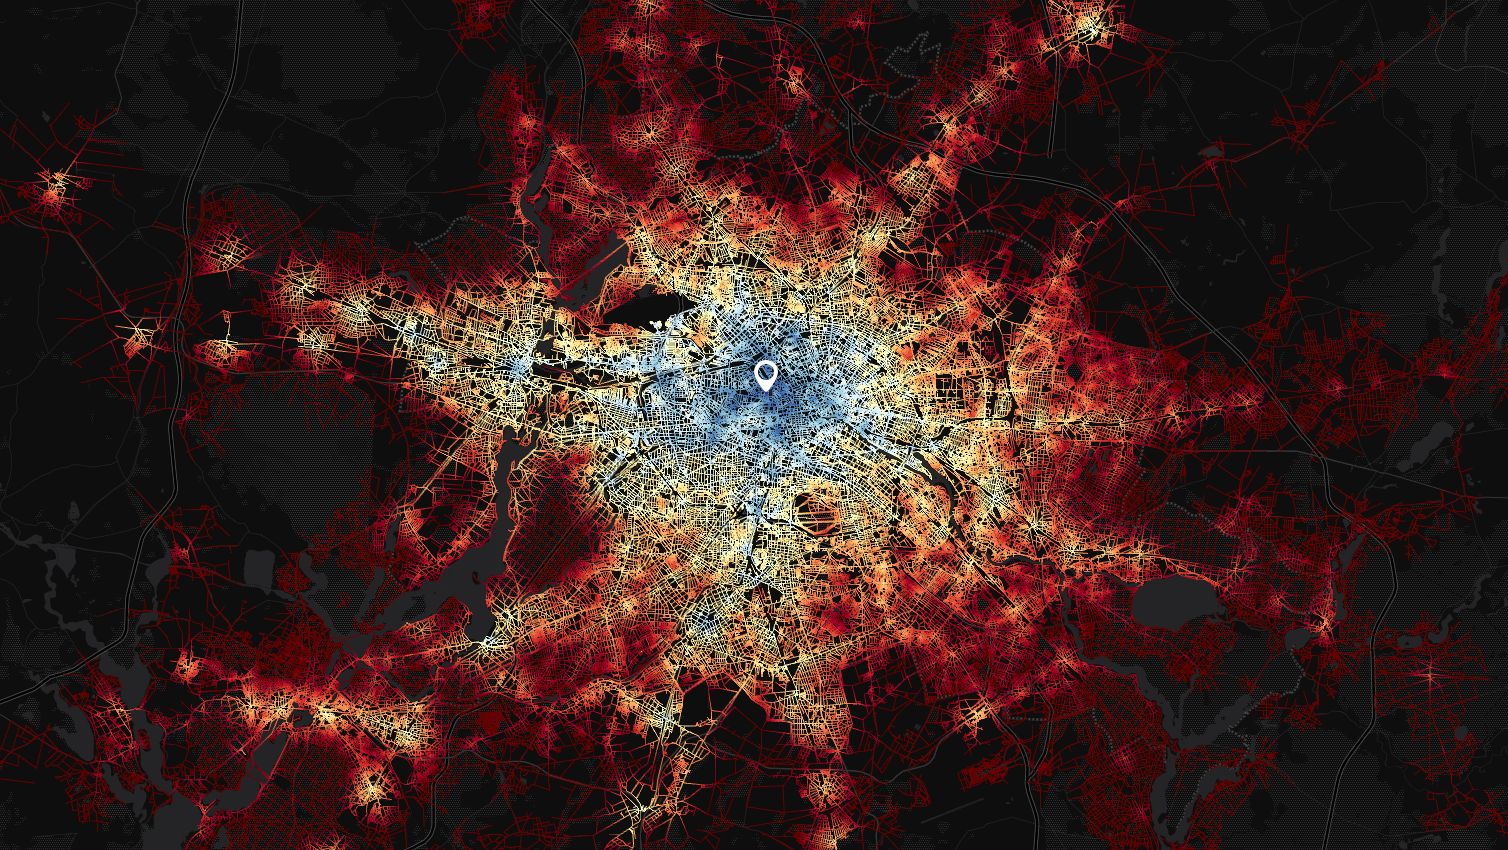
\includegraphics[width=\linewidth]
        {./img/screenshot-teaser-7200s-publictransport.png}
      \caption{A network-based accessibility map visualization.}
      \label{fig:intro:teasr}
    \end{figure}

    However, these techniques do not supply a convenient approach to map and
    render high detailed, unfiltered transportation network geometries
    required for applications such as accessibility analytics (compare Figure
    \ref{fig:intro:teasr}).\par

  \section{Definitions}
    \label{sec:intro:def}

    Both the terms \textit{transportation networks} and \textit{accessibility
    maps} are ambiguous and will be defined for future usage in this
    thesis.\par

    \begin{description}
      \item[Transportation Network] is a multimodal, routable graph
        representation of a geographic dataset.
        It includes all types of roads from motorways to residential paths
        including foot-ways and cycle-ways [??]. It does not include railways or
        bus guide-ways which are not accessible by private means of transport.
      \item[Accessibility Maps] are tools for mobility analytics. They display
        single source shortest path (\acrshort{sssp}) routing for selected
        geographic areas [??]. Accessibility can used be as a synonym for
        \textit{reachability} in this case. It's not related to services or
        environments for people who experience disabilities.

        % term accessibility Hansen (1959)
        % reachability analysis in Innerebner (2013)
        % travel time maps in Campenhout (2010)
        % both Yin (2015)

    \end{description}

  \section{Problem statement}
    \label{sec:intro:probl}

    Figure \ref{fig:intro:r360d} shows an existing web service for accessibility
    mapping. It encodes travel time intervals using separate polygons, which
    must be computed and transferred to the browser. This kind of approach has
    several drawbacks:\par

    \begin{enumerate}[\label=({D}1)]
      \item \label{enu:drawb:d1} It's creation requires generalization.
      \item \label{enu:drawb:d2} It lacks precision with regard to the network.
      \item \label{enu:drawb:d3} It does not scale for a more detailed display.
    \end{enumerate}

    \begin{figure}[htb]
      \centering
      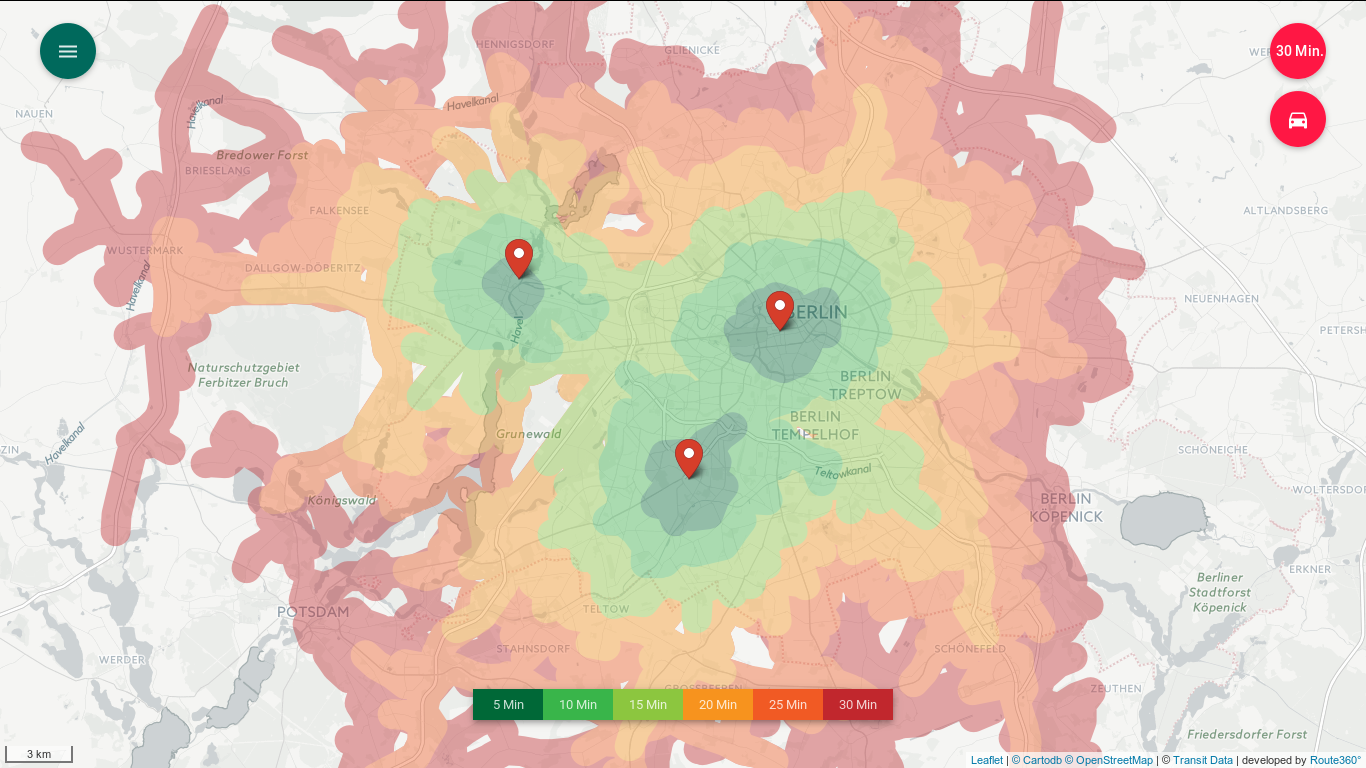
\includegraphics[width=\linewidth]
        {./img/screenshot-r360js-demo.png}
      \caption{A generalized, polygon-based accessibility map visualization
        by Motion Intelligence GmbH utilizing the Route360$^\circ$-\acrshort{js}
        \acrshort{api} [??].}
      \label{fig:intro:r360d}
    \end{figure}

    Real-time rendering transportation networks as scenery for data
    visualization in web-based applications is a performance critical task
    depending on the geometric complexity of the network and associated travel
    times. For example, an OpenStreetMap (\acrshort{osm}) dataset of the Berlin
    region comprises approximately $2.4 \cdot 10^6$ road segments spanned by
    $2.9 \cdot 10^6$ vertices as of June 2016 [??]. Traditional visualization
    approaches using web browsers either face users with a predefined, static
    filtering and mapping (raster data) or a notable computation-intense
    rendering process (vector data). These two fundamental approaches covering
    filtering, mapping, and rendering web-based maps are widely established and
    have proven to be effective, but exhibit additional drawbacks.\par

    Data transmitted in pre-rendered raster data formats (e.g., \acrshort{png},
    \acrshort{jpg}) do
    not require any client-side processing prior to rendering, can be compressed
    as well as cached~\cite{ESRI2006}, and is used by major web-mapping services
    such as Google or Bing maps [??]. However, one major disadvantage is the
    lack for client-side filtering and mapping without requesting a complete map
    tile reload. Web services using this technology approach this by using small
    vector overlays displaying additional user-styled information [??], but it
    is not possible to access the the map data itself.\par

    In contrast thereto, geo-data transmitted using vector formats
    (e.g., \acrshort{json}, \acrshort{gml}) enable
    client-side filtering, mapping, and rendering. This client-side processing
    however introduces a major performance impact: both the data processing and
    rendering are usually performed on central processing units (\acrshort{cpu})
    using JavaScript (\acrshort{js}) algorithms. Recent approaches do support
    hardware-accelerated rendering (\acrshort{gpu}) but lack functionality for
    client-side vector data processing~\cite{Gaffuri2012}.\par

    Thus, both approach changes in filtering (e.g., selecting a travel time
    threshold) or mapping (e.g., color mapping, line styles etc.) would result
    in a complete data re-transmission, loading, and processing.\par

    Therefore, high detailed network analysis and visualization is often
    performed using Geographic Information Systems (\acrshort{gis}) [??]. Such
    systems
    exploit the computation power of desktop workstations but posses limited
    applicability to everyday life, due to data availability and access, as well
    as expert domain knowledge required by a user [??].\par

  \section{Contributions}
    \label{sec:intro:contr}

    In the light of powerful, dedicated graphics hardware being not only
    available on personal computers (\acrshort{pc}) but also
    on small, mobile devices nowadays, this thesis suggests new techniques for
    client-side rendering of web-maps with complex geometries on graphic
    processing units (\acrshort{gpu}).\par

    The challenge of this work is twofold interesting. On the one hand it is
    important to enable rendering using GPU-based techniques like
    the web graphics library (\acrshort{webgl}) \cite{Jackson2016}.
    This allows dynamic, interactive and user-defined styles to be rendered
    directly on the client's device. But on the other hand it is a must to
    completely eliminate the client-side mapping of the geo-data as this becomes
    a major performance bottleneck with increasing data complexity.\par

    This thesis proposes a new approach for web-based visualization of
    accessibility maps based on transportation network data. This geometry-based
    approach uses vector data (lines) stored and transmitted using the new
    standardized graphics library transmission format (\acrshort{gltf}) [??],
    which reduces performance-critical
    computations in the visualization client (i.e., coordinate transformations)
    and thus facilitates real-time rendering with high run-time performance
    yielding low client response times. To summarize, this work makes the
    following contributions:\par

    \begin{enumerate}[\label=({C}1)]
      \item \label{enu:contr:c1} It presents a concept to decouple the
        visualization geometry and data items for interactive web-based
        accessibility maps based on \acrshort{webgl}.
      \item \label{enu:contr:c2} It specifies a geographic tiling concept based
        on a binary transmission format close to rendering requirements
        utilizing the new standardized \acrshort{gltf}.
      \item \label{enu:contr:c3} It demonstrates the effectiveness of this
        approach by a comparative performance evaluation of different
        implementation variants.
    \end{enumerate} % @TODO compare innereber thesis 2013

    The technique presented in this thesis is a graphics library (\acrshort{gl})
    based approach rather than classic vector- or raster-based provisions.
    It shows various advantages:\par

    \begin{enumerate}[\label=({A}1)]
      \item \label{enu:advnt:a1} Its usage is not limited to stationary desktop
        systems but available on a variety of devices (esp. mobile).
      \item \label{enu:advnt:a2} Potentially massive data sources are not
        required to be completely transmitted, stored, or managed.
      \item \label{enu:advnt:a3} Implementations based on web-services and
        \acrshort{webgl} can be easily integrated into existing systems and
        visualization frameworks.
    \end{enumerate}

    In contrast to existing accessibility-map visualization concepts, this work
    focuses on visualizing the travel time data directly on the respective
    transportation network features, rather than (possibility generalized)
    polygons~\cite{Glander2010} or specific graph layouts~\cite{Krause2012}.
    This enables a precise mapping of travel data to the geo-referenced
    transportation network. However, considering the high geometric complexity
    (vertices, primitives) introduced by increasing quality of transportation
    networks~\cite{Zielstra2010}, e.g., of massive open data transportation
    networks (OpenStreetMap (\acrshort{osm}) or General Transit Feed
    Specification (\acrshort{gtfs})),
    an implementation of an interactive web-based visualization technique
    comprises a number of conceptual and technical challenges.\par

    It maintains the goal to allow real-time rendering with outstanding
    performance and very low response times for the client.\par


  \section{Publications}
    \label{sec:intro:publc}
    \begin{itemize}
      \item \textsc{Schoedon, A; Trapp, M; Hollburg, H; Döllner,
        J (2016)}:\\ Interactive Web-based Visualization for Accessibility
        Mapping of Transportation Networks. In: Eurographics Conference on
        Visualization (\textsc{EuroVis}) 2016, The Eurographics Association,
        Groningen \cite{STHD2016}.
    \end{itemize}

  \section{Thesis Organization}
    \label{sec:intro:organ}
    Chapter \ref{chap:overv} provides an overview on accessibility mapping and
    mobility analytics, on geographic visualizations of transportation networks,
    of web-based mapping components and services, and web-based rendering
    technologies.\par

    Chapter \ref{chap:requr} defines the requirements for this approach, while
    chapter \ref{chap:conct} presents the concept and explains the design
    decisions made.\par

    Chapter \ref{chap:imple} outlines the different proof-of-concept
    applications and explains the architecture and important implementation
    details with respect to the requirements.\par

    While chapter \ref{chap:evalu} shows application examples in coorperation
    with Motion Intelligence GmbH and a performance evaluation, a discussion of
    the results can be found in chapter \ref{chap:discu}.\par
